\section{Fluxograma do jogo}

A Figura \ref{figura:fluxograma} detalha o fluxo do jogo com as ações possivelmente executadas pelos jogadores.

\begin{center}
	\includegraphics[scale=0.5]{figuras/fluxograma}
	\captionof{figure}{Fluxograma do Jogo.}
	\label{figura:fluxograma}
\end{center}

\section{Funcionalidades}
\subsection{Menu}
O menu é o módulo pelo qual o usuário irá escolher suas opções de jogo, sendo elas: a criação de conta ou a utilização de uma já existente, escolha dos modos de jogo, seleção de número de voltas na pista, escolha da pista, cenário noturno ou diurno, visualização de gráficos. Esta sequência de escolhas no menu possibilitará ao jogador diferentes versões de ambientes de realidade virtual.

\begin{center}
	\includegraphics[scale=0.4]{figuras/play}
	\captionof{figure}{Tela inicial do menu.}
	\label{figura:play}
\end{center}

\begin{center}
	\includegraphics[scale=0.4]{figuras/name}
	\captionof{figure}{Tela de inserir o nome para criar conta.}
	\label{figura:name}
\end{center}

\begin{center}
	\includegraphics[scale=0.4]{figuras/numerodevoltas}
	\captionof{figure}{Tela de selecionar o número de voltas.}
	\label{figura:numVoltas}
\end{center}

\subsection{Modo Corrida}
\label{corrida}

Para cada cenário disponível no jogo é possível escolher dentre dois modos: um deles é o modo corrida e outro é o modo livre. A principal diferença presente é a restrição do número de voltas no circuito no modo corrida. Contudo, outras particularidades são encontradas nesse modo, como a contabilização do tempo, a restrição do sentido da bicicleta para computação das voltas e delimitação do cenário do circuito, para auxiliar o cumprimento das voltas.

Depois de escolher o pista que deseja, o usuário escolhe a quantidade de voltas que vai correr e então começa a corrida. O início e o fim do modo corrida são demarcados pela linha de chegada (Figura \ref{figura:linhadechegada}). O modo corrida termina assim que as voltas acabam, e então é mostrado o seu desempenho.

\begin{center}
	\includegraphics[scale=0.4]{figuras/linhadechegada}
	\captionof{figure}{Linha de Chegada.}
	\label{figura:linhadechegada}
\end{center}

\subsection{Modo Livre}
\label{livre}
Diferentemente da funcionalidade anterior, o modo livre tem o propósito de deixar o usuário experimentar o ambiente virtual criado. Nenhuma das particularidades citadas anteriormente está presente nele. Para iniciá-lo é necessário apenas escolher a pista que deseja explorar. A partir de então é iniciado o modo livre. Ele só acaba quando é pausado o jogo. Sendo que tal interação se dá quando o usuário tira alguma de suas mãos do guidão da bicicleta física. Neste momento é mostrado então a opção de se encerrar o modo livre.

\subsection{Controle da Bicicleta}
Essa funcionalidade descreve a comunicação do sistema eletrônico, que devolve dados de velocidade da bicicleta e rotação do guidão. Com esses dados, o jogo deve ser capaz de controlar a bicicleta no cenário, alterando a velocidade do objeto, movimentando o sistema personagem-bicicleta-câmeras e rotacionando a direção do jogador, além de rotacionar o guidão para fidelidade visual.

\subsection{Física do Jogo}
A física do jogo é a parte responsável pela detecção e tratamento das colisões entre os objetos físicos dele. Nesse jogo, é necessário definir um poliedro de colisão para a bicicleta, de forma que fique realista a um nível em que o jogador tenha a sensação de estar em uma bicicleta real. Além de poliedros de colisão para a grama, as pistas, a cerca e a linha de chegada. Essas colisões são tratadas pela \textit{Unity} e podem ser capturadas por código para mudar estados e ativar sons, como batida em cerca e caminhada na grama.

\subsection{Conta}
A fim de conseguir customizar a experiência de cada usuário, o jogo consta com a funcionalidade de criação de uma conta. Assim que é ele entra no jogo é possível selecionar uma conta já existente ou criar uma nova. Para criar a conta é necessário informar o nome, peso, altura e sexo. A partir de então, com a conta criada é possível acessar as outras funcionalidades, bem como acessar algumas estatísticas próprias do jogo. Por final, é possível na tela de criar uma conta deletar uma já existente.

\subsection{Gráficos}
Além dos dados já informados pelo próprio usuário ao criar a sua conta, a plataforma possui sensores que irão coletar e medir dados como velocidade da bicicleta, batimentos cardíacos, resistência galvânica da pele, frequência respiratória, entre outros. Durante o jogo serão exibidos alguns destes dados coletados como ilustrado na Figura \ref{figura:canvas} e ao final serão exibidos de forma mais detalhada. Estes dados de cada corrida serão armazenados na conta do usuário e possibilitarão a ele a visualização de gráficos que servirão para demonstrar o seu desempenho na plataforma.

\begin{center}
	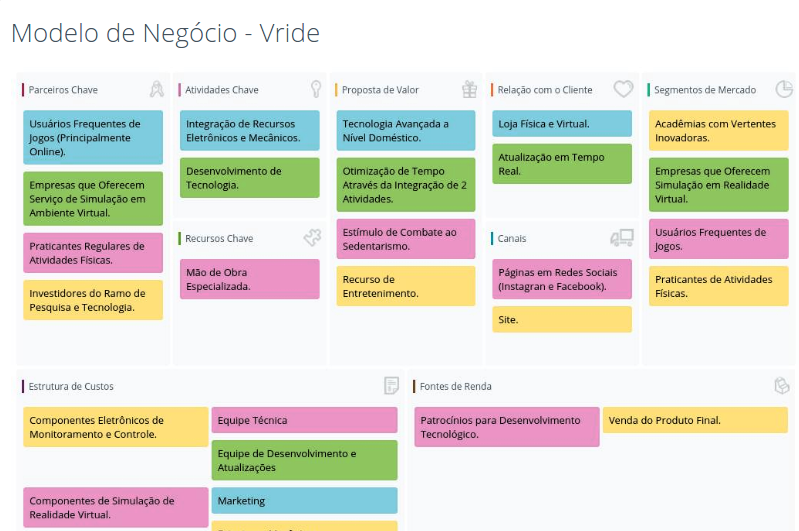
\includegraphics[scale=0.4]{figuras/canvas}
	\captionof{figure}{Informações do Modo Corrida.}
	\label{figura:canvas}
\end{center}

\subsection{Personagens}
A visão do jogador consiste na orientação da câmera que representa o \textit{Oculus}. Dentro do jogo é a visão do personagem, no qual está posicionado em cima da bicicleta, para proporcionar a sensação de imersão. É possível visualizar a movimentação do personagem como o pedalar de acordo com a velocidade, os braços acompanhando a direção do guidão, entre outras. Existem dois tipos de personagens no jogo que podem ser selecionados pelo jogador: um homem e uma mulher, demonstrados nas (Figuras \ref{figura:mulher} e \ref{figura:homem}) .

\begin{center}
	\includegraphics[scale=0.4]{figuras/mulher}
	\captionof{figure}{Personagem feminina vista de perfil.}
	\label{figura:mulher}
\end{center}

\begin{center}
	\includegraphics[scale=0.4]{figuras/homem}
	\captionof{figure}{Personagem feminina vista de perfil.}
	\label{figura:homem}
\end{center}

\subsection{Cenários}

O jogador poderá escolher opções do cenários para jogar como:

\begin{description}
\item[Pistas] Uma pista íngreme e uma pista regular.
\item[Modo Corrida e Modo Livre] Detalhados nas Seções \ref{corrida} e \ref{livre}.
\item[Noturno e Diurno] Cenário noturno (Figura \ref{figura:noturno}) com os postes ligados, lua e estrelas e o cenário diurno (Figura \ref{figura:diurno}) com nuvens, sol e postes desligados.
\end{description}

\begin{center}
	\includegraphics[scale=0.4]{figuras/noturno}
	\captionof{figure}{Cenário noturno.}
	\label{figura:noturno}
\end{center}

\begin{center}
	\includegraphics[scale=0.4]{figuras/diurno}
	\captionof{figure}{Cenário diurno.}
	\label{figura:diurno}
\end{center}

As imagens abaixo contém os elementos principais que compõem o cenário do jogo.

\begin{center}
	\includegraphics[scale=0.4]{figuras/pista}
	\captionof{figure}{Vista superior da pista regular.}
	\label{figura:pista}
\end{center}

\begin{center}
	\includegraphics[scale=0.4]{figuras/jardim}
	\captionof{figure}{Jardim localizado no centro do cenário.}
	\label{figura:jardim}
\end{center}


\begin{center}
	\includegraphics[scale=0.4]{figuras/torcida}
	\captionof{figure}{Torcida localizada proximo à linha de chegada.}
	\label{figura:torcida}
\end{center}

\begin{center}
	\includegraphics[scale=0.4]{figuras/visaocima}
	\captionof{figure}{Visão próxima á linha de chegada.}
	\label{figura:visaodecima}
\end{center}

\section{Arquitetura}

\subsection{Modelo de Domínio}

O modelo de domínio representado nas (Figuras \ref{figura:menu_domain} e \ref{figura:main_domain}) faz referência aos dois módulos principais do desenvolvimento do jogo. O menu sendo representado por todos os componentes que interagem com o usuário para que ele escolha o modo de jogo e pelos componentes que armazenam informações do usuário. E o \textit{Simple Track Run} que engloba os componentes utilizados na construção do percurso que o usuário irá fazer ao jogar, como os cenários, personagens, torcida.

\begin{center}
	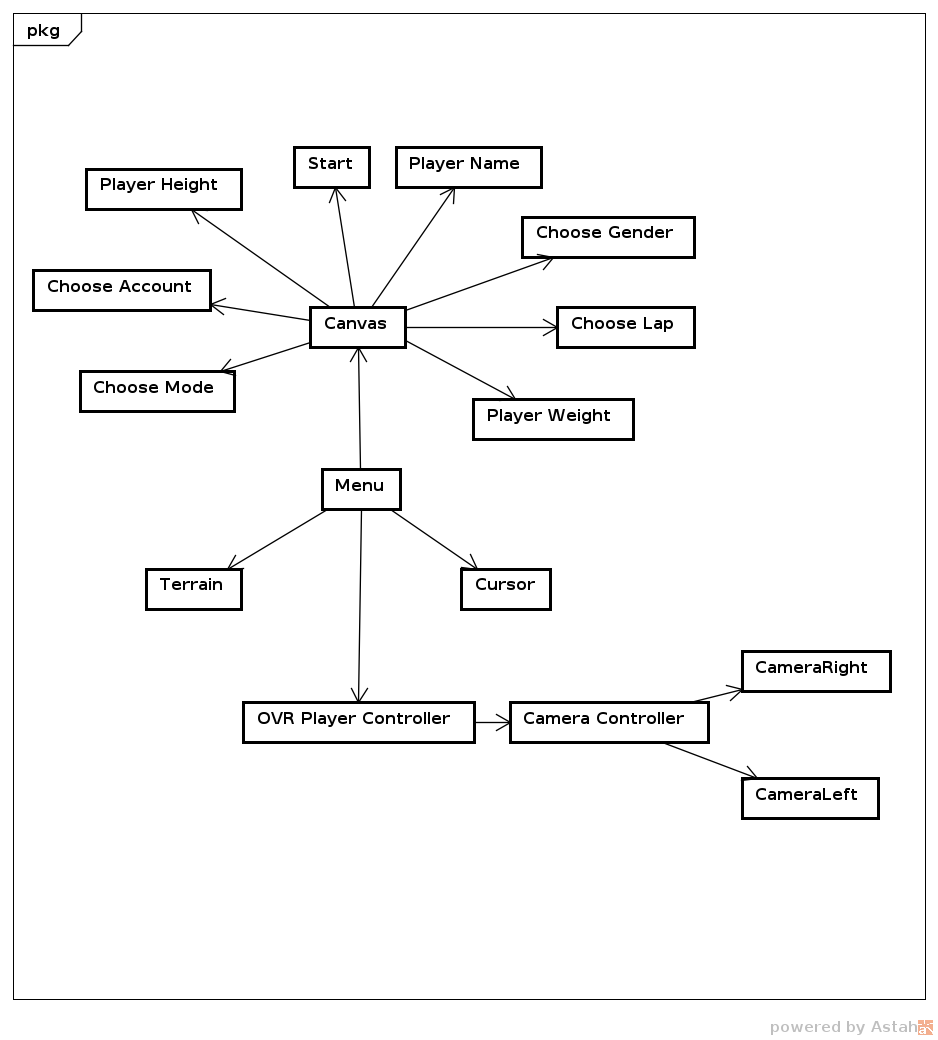
\includegraphics[scale=0.5]{figuras/menu_domain}
	\captionof{figure}{Modelo de Domínio - Menu.}
	\label{figura:menu_domain}
\end{center}

\begin{center}
	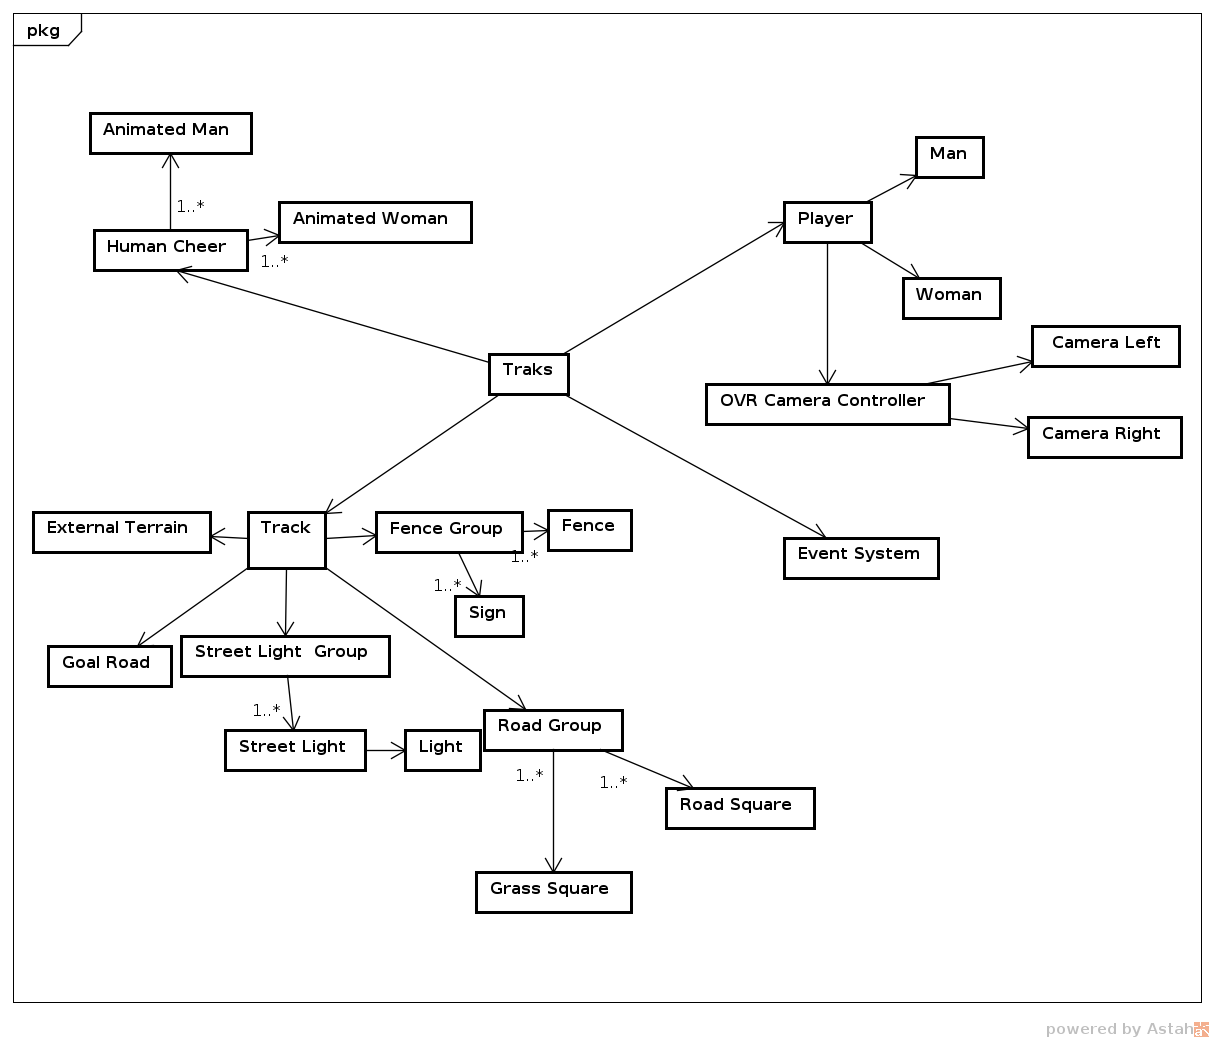
\includegraphics[scale=0.5]{figuras/main_domain}
	\captionof{figure}{Modelo de Domínio - \textit{Simple Track Run}.}
	\label{figura:main_domain}
\end{center}

\subsection{Arquitetura de Componentes}

A \textit{Unity 3D} possui uma arquitetura baseada em componentes. Tal decisão arquitetural é baseada no princípio de que os objetos de um jogo - como personagem, árvore, chão - são formados por diversos componentes diferentes - como imagem, som, colidível e outros. Dessa forma, ao invés de cada tipo de objeto do jogo possuir novas funcionalidades por meio de herança, novos componentes são adicionados a eles de forma dinâmica. Na \textit{Unity}, em específico, cada objeto herda da classe \textit{GameObject} que possui métodos de adicionar e remover componentes. Todos os componentes herdam da classe \textit{Component} e alguns dos mais usados incluem:

\begin{itemize}
\item \textit{Collider}: Adiciona uma área de colisão ao objeto, que pode reagir a colisões físicas ou de gatilho em métodos como \textit{OnCollisionEnter} e \textit{OnTriggerEnter};
\item \textit{AudioSource:} Adiciona som ao objeto, que pode tocar, automaticamente, em \textit{loop} e ser 3D (ter uma fonte espacial no jogo) ou não.
\item \textit{Transform}: Guarda as informações acerca da posição e da rotação de um objeto.
\item \textit{Script}: Adiciona instruções ao objeto. Podem ser escritos em C\# ou \textit{Javascript}, com instruções executadas ao iniciar (\textit{Start}), a cada \textit{frame} (\textit{Update}) ou em determinados eventos (\textit{OnCollisionExit} e outras).
\end{itemize}

Em relação à construção do jogo, os menus e fases são agrupados em cenas (\textit{scenes}). Cada cena possui uma hierarquia com diversos \textit{game objects}. Cada \textit{game object} possui um pai e um ou mais filhos. A cada \textit{frame}, todos os \textit{game objects} são atualizados e todos os métodos de \textit{update} dos \textit{scripts} executados.

\begin{center}
	\includegraphics[scale=0.4]{figuras/arquiteturacomponentes}
	\captionof{figure}{Arquitetura de Componentes. Fonte: \cite{arquitetura}}
	\label{figura:arquiteturacomponentes}
\end{center}

\subsubsection{\textit{Scripts}}

Os \textit{scripts} são a parte em que os desenvolvedores alteram o comportamento do jogo programaticamente. Cada \textit{script} altera o comportamento de um \textit{game object} diretamente e pode alterar o de outros de forma indireta. Cada \textit{game object} pode ter um ou mais scripts.

Os principais scripts do jogo são:

\begin{itemize}
\item \textit{PlayerScript}: Responsável pelo controle do jogador, utilizando os valores de velocidade e rotação para movimentar a bicicleta, o personagem e a câmera.
\item \textit{HandleBarScript}: Responsável pela rotação do guidão da bicicleta de acordo com a rotação recebida da classe InputOutput.
\item \textit{Scripts} de áudio: Responsáveis pela reprodução de áudio de colisão com cercas e chão, reproduzindo sons característicos em tal contato.
\item \textit{CheeringScript}: Responsável pelo início da animação dos personagens de torcida para que eles não tenham a animação sincronizada, mas em tempos randômicos em relação um ao outro.
\item \textit{Scripts} do menu: Responsáveis pela transição dos paíneis dentro do menu, pelo controle das ações e comportamento dos botões e por salvar e carregar as informações da conta.
\end{itemize}

\subsection{Fluxo de Informa\c{c}ões}
\subsubsection{MQTT}

O MQTT é um protocolo baseado em mensagens utilizado em soluções IOT. Como ilustrada na Figura \ref{figura:mqttsoft}, o MQTT possui três papéis principais para o estabelecimento das trocas de mensagens: o \textit{Broker}, o \textit{Publisher} e o \textit{Subscriber}: O \textit{Broker} é um servidor responsável por intermediar o recebimento e envio das mensagens e é onde é implementado toda a lógica responsável pelo armazenamento de dados. O \textit{Publisher} é o dispositivo que mandará mensagens em tópicos para o Broker de modo que fique acessível para o \textit{Subscriber} ler a mensagens.

A identificação das mensagens é definida por tópicos que podem ser identificadas por palavras divididas por barras, como por exemplo: \textit{\textbf{bike/velocity}}. Para que o \textit{Publisher} publique uma mensagem, o tópico deve ser definido. E para que o \textit{Subscriber} leia a mensagem, ele se inscrever no tópico desejado. Os dados contidos nas mensagens trocadas pelo MQTT estão em \textit{bytecode}.

\begin{center}
	\includegraphics[scale=0.4]{figuras/MQTT}
	\captionof{figure}{Fluxo de mensagens do MQTT.}
	\label{figura:mqttsoft}
\end{center}


Neste projeto, o jogo agirá como um \textit{Publisher} e como um \textit{Subscriber}. Por exemplo, para definir a velocidade da bicicleta e a angulação do guidão, agirá como um \textit{Subscriber} e para definir a angulação vertical, agirá como um \textit{Publisher}. As funções de publicação, inscrição, conexão, entre outras é importada do asset do MQTT disponível para Unity.  A classe que faz as intermediações entre os dados no jogo é a \textit{InputOutput} que será detalhada no tópico a seguir.

\subsubsection{\textit{InputOutPut} e \textit{Mock} do \textit{Input}}

Na função \textit{Start} da classe  \textit{InputOutput}, é realizada a conexão do jogo com o \textit{Broker} através do IP e porta e a inscrição de todos os tópicos que serão utilizados. Os tópicos presentes atualmente são: o \textit{bike/velocity} para a velocidade da bicicleta e o \textit{bike/angle} para a angulação do guidão.

Como a integração com o sistema físico ainda não foi realizada, é implementado um \textit{Publisher} para enviar mensagens a partir de eventos do teclado. Portanto, para testes do subsistema isolado, o fluxo de informações é o seguinte:

\begin{itemize}
\item Quando a seta ${\uparrow}$ é pressionada, é enviado uma mensagem através de um Publish que a tecla está sendo pressionada no tópico \textit{bike/velocity} . No \textit{script} responsável pelo controle do movimento da bicicleta, são repassadas as mensagens contidas no tópico de velocidade que aumenta gradativamente enquanto esta tecla estiver pressionada.
\item Quando as setas ${\leftarrow}$ e ${\rightarrow}$ são pressionadas, também é enviado uma mensagem através de um \textit{Publish} que a tecla está sendo pressionada no tópico \textit{bike/angle}. As mensagens contidas no tópico de angulação são repassadas para o script responsável pela movimentação e é variada então em 45$^{\circ}$  para direita ou esquerda dependendo da tecla pressionada e para 0$^{\circ}$  quando nenhuma das duas estiver pressionada.
\item Concluindo, o \textit{Publisher} que é acionado através do \textit{Input.GetKey}, uma espécie de handler de eventos do teclado,  envia dados para o \textit{Broker} que repassa para o jogo como demonstrado na Figura \ref{figura:inputoutput}.
\end{itemize}

\begin{center}
	\includegraphics[scale=0.4]{figuras/inputoutp}
	\captionof{figure}{Integração através do MQTT}
	\label{figura:inputoutput}
\end{center}

\subsection{Banco de Dados}
Para o armazenamento das informações relativas a conta de um usuário foi adotado a utilização de um banco de dados. Tais informações incluem tanto os dados pessoais como, nome, altura e peso, quanto os dados relativos ao desenvolver do usuário, como o tempo das voltas, batimentos cardíacos durante a corrida, frequência respiratória e velocidade no circuito, entre outros, que poderão vir a ser adicionados para melhorar a funcionalidade de estatísticas.

O banco de dados escolhido foi o \textit{iBoxBD} (\url{http://www.iboxdb.com/}), uma banco de bados totalmente não relacional, que é leve e usa pouca memória. Ele é executado como um servidor incorporado como banco de dados local, também suporta conexão TCP como parte do sistema distribuído. Outras vantagens são: único arquivo, ausência da necessidade de configuração e suporte ao C\#.

Na implementação dele no projeto foi criado um \textit{Singleton}, que instância e gerencia a \textit{“Box”}, que é parte desse BD que cuida do contexto das operações e as executa. Além disso foi criada uma DAO para a classe \textit{Player} e para a \textit{Measure}, que separa as regras de negócio do jogo do acesso aos dados, que se dá pelo \textit{Singleton}. Na figura \ref{figura:banco_de_dados} é possível visualizar o que o banco de dados guarda atualmente.

\begin{center}
	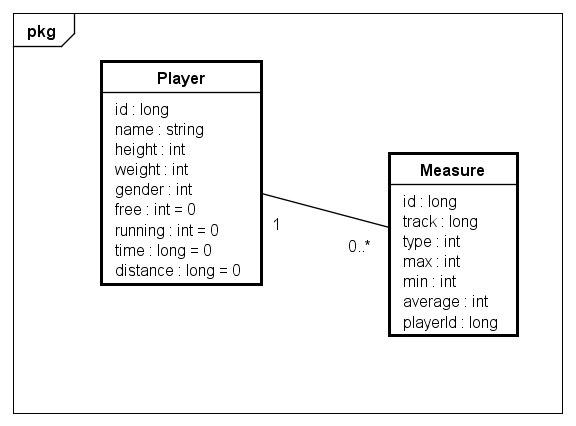
\includegraphics[scale=0.6]{figuras/banco_de_dados}
	\captionof{figure}{Diagrama de classe das entidades do Banco de Dados}
	\label{figura:banco_de_dados}
\end{center}

Por ser um banco de dados não relacional, o relacionamento representado no diagrama \ref{figura:banco_de_dados} não é realizado por meio de chaves estrangeiras, e sim por um único índice presente na classe \textit{Measure} pelo \textit{playerId}. Essa entidade guarda as informações referentes as medidas que são aferidas durante o jogo. Para não onerar o banco de dados, a cada corrida é calculado o valor médio e identificado o valor mínimo e máximo. O \textit{type} nesse caso guarda o tipo de medida que está sendo guardada, sendo referente ao Enum \textit{Type} presente nessa mesma classe.

A classe \textit{Player} ainda guarda informações como o tempo total de jogo, a distância percorrida e a quantidade de corrida realizada em cada modo de jogo.

\section{Métricas de Código}

Ao decorrer do projeto viu-se a necessidade de se coletar métricas principalmente para averiguar se o código está em boas condições para que seja manutenido e evoluído. Para isso, foi escolhido algumas métricas, que serão explicadas posteriormente, do \textit{Analizo} disponibilizas para a linguagem Java/C++.

Os indicadores propostos tem como base um artigo sobre o \textit{kalibro} \cite{dekalibro}. Procurou-se observar níveis que vão garantir o objetivo estipulado de qualidade de código. A tabela \ref{metricas_descricao} apresenta as métricas escolhidas.

\begin{table}[htp]
\centering
\caption{Indicadores}
\label{metricas_descricao}
\begin{tabular}{|c|c|c|c|}
\hline
\textbf{Métrica}                                                                                                                         & \textbf{Código} & \textbf{Descrição}                                                                                                                                                                                                                                                & \textbf{Indicadores}                                                                                  \\ \hline
\begin{tabular}[c]{@{}c@{}}\textit{Average Cyclomatic} \\ \textit{Complexity per Method} \\ (Média de complexidade \\ ciclomática por método)\end{tabular} & accm            & \begin{tabular}[c]{@{}c@{}}Complexidade ciclomática nada\\  mais é do que o número de \\ caminhos independentes que um \\ software pode seguir \\ em sua execução, \\ calculado a partir da\\  representação em grafo \\ das estruturas de controle.\end{tabular} & \begin{tabular}[c]{@{}c@{}}Bom {[}0, 5{[}\\ Regular {[}5, 7{[}\\ Ruim {[}7, INF{[}\end{tabular}       \\ \hline
\begin{tabular}[c]{@{}c@{}}\textit{Average Method} \\ \textit{Lines of Code} \\ (Média de linhas de \\ código por método)\end{tabular}                     & amloc           & \begin{tabular}[c]{@{}c@{}}AMLOC representa a média\\  do número de linhas dos\\  métodos de uma classe.\end{tabular}                                                                                                                                             & \begin{tabular}[c]{@{}c@{}}Bom {[}0, 10{[}\\ Regular {[}10, 13\\ {[}Ruim {[}13, INF{[}\end{tabular}   \\ \hline
\begin{tabular}[c]{@{}c@{}}\textit{Lack of Cohesion} \\ \textit{of Methods}\\ (Ausência de coesão \\ em métodos)\end{tabular}                              & lcom4           & \begin{tabular}[c]{@{}c@{}}LCOM4 representa a coesão \\ entre os métodos da classe.\\  Ela verifica a relação entre os\\  métodos e atributos de uma \\ mesma classe.\end{tabular}                                                                                & \begin{tabular}[c]{@{}c@{}}Bom {[}0, 2{[}\\ Regular {[}2, 5{[}\\ Ruim {[}5, INF{[}\end{tabular}       \\ \hline
\begin{tabular}[c]{@{}c@{}}\textit{Lines of Code}\\ (Linhas de código\\  por classe)\end{tabular}                                                 & loc             & \begin{tabular}[c]{@{}c@{}}LOC indica o número de linhas\\  executáveis de uma classe, \\ desconsiderando linhas \\ em branco e comentários.\end{tabular}                                                                                                         & \begin{tabular}[c]{@{}c@{}}Bom {[}0, 70{[}\\ Regular {[}70, 130{[}\\ Ruim {[}130, INF{[}\end{tabular} \\ \hline
\begin{tabular}[c]{@{}c@{}}\textit{Number of Methods}\\ (Número de métodos)\end{tabular}                                                          & nom             & \begin{tabular}[c]{@{}c@{}}NOM é uma métrica de \\ tamanho que conta o \\ número de métodos \\ de uma classe.\end{tabular}                                                                                                                                        & \begin{tabular}[c]{@{}c@{}}Bom {[}0, 10{[}\\ Regular {[}10, 40{[}\\ Ruim {[}40, INF{[}\end{tabular}   \\ \hline
\end{tabular}
\end{table}

A partir das métricas escolhidas foi realizado a coleta dos dados e análise com base nos indicadores. A tabela \ref{figura:metricas} apresenta os \textit{scripts} que foram criados e os valores referentes para cada métrica. A coloração de cada célula foi realizada para melhor representar a situação de cada um, sendo que o verde significa bom, o amarelo significa regular e o laranja significa ruim.

\begin{table}[htp]
\centering
\caption{Métricas de Código}
\label{figura:metricas}
\begin{tabular}{lllllll}
\hline
Script & ACCM & AMLOC & LCOM4 & LOC & NOM \\
\hline
CameraMovementScript.cs & 4.25\cellcolor[HTML]{9AFF99} & 23.375\cellcolor[HTML]{FFCE93} & 2\cellcolor[HTML]{FFFC9E} & 187\cellcolor[HTML]{FFCE93} & 0\cellcolor[HTML]{9AFF99} \\
CheeringScript.cs & 2.5\cellcolor[HTML]{9AFF99} & 8.5\cellcolor[HTML]{9AFF99} & 1\cellcolor[HTML]{9AFF99} & 17\cellcolor[HTML]{9AFF99} & 2\cellcolor[HTML]{9AFF99} \\
FenceAudioScript.cs & 1\cellcolor[HTML]{9AFF99} & 4.5\cellcolor[HTML]{9AFF99} & 1\cellcolor[HTML]{9AFF99} & 9\cellcolor[HTML]{9AFF99} & 2\cellcolor[HTML]{9AFF99} \\
GrassAudioScript.cs & 1.2857\cellcolor[HTML]{9AFF99} & 4.2857\cellcolor[HTML]{9AFF99} & 1\cellcolor[HTML]{9AFF99} & 30\cellcolor[HTML]{9AFF99} & 7\cellcolor[HTML]{9AFF99} \\
HandleBarScript.cs & 1\cellcolor[HTML]{9AFF99} & 4\cellcolor[HTML]{9AFF99} & 2\cellcolor[HTML]{FFFC9E} & 8\cellcolor[HTML]{9AFF99} & 2\cellcolor[HTML]{9AFF99} \\
InputOutput.cs & 1.875\cellcolor[HTML]{9AFF99} & 11\cellcolor[HTML]{FFFC9E} & 3\cellcolor[HTML]{FFFC9E} & 176\cellcolor[HTML]{FFCE93} & 16\cellcolor[HTML]{FFFC9E} \\
KneeScript.cs & 1\cellcolor[HTML]{9AFF99} & 3.5\cellcolor[HTML]{9AFF99} & 1\cellcolor[HTML]{9AFF99} & 7\cellcolor[HTML]{9AFF99} & 2\cellcolor[HTML]{9AFF99} \\
AccountDelete.cs & 1.8\cellcolor[HTML]{9AFF99} & 6.8\cellcolor[HTML]{9AFF99} & 2\cellcolor[HTML]{FFFC9E} & 34\cellcolor[HTML]{9AFF99} & 5\cellcolor[HTML]{9AFF99} \\
AccountSelect.cs & 1.4285\cellcolor[HTML]{9AFF99} & 6.7142\cellcolor[HTML]{9AFF99} & 2\cellcolor[HTML]{FFFC9E} & 47\cellcolor[HTML]{9AFF99} & 7\cellcolor[HTML]{9AFF99} \\
CountLaps.cs & 1.8\cellcolor[HTML]{9AFF99} & 6.6\cellcolor[HTML]{9AFF99} & 2\cellcolor[HTML]{FFFC9E} & 33\cellcolor[HTML]{9AFF99} & 5\cellcolor[HTML]{9AFF99} \\
IgnoreRaycast.cs & 1\cellcolor[HTML]{9AFF99} & 4\cellcolor[HTML]{9AFF99} & 1\cellcolor[HTML]{9AFF99} & 4\cellcolor[HTML]{9AFF99} & 1\cellcolor[HTML]{9AFF99} \\
LoadLevel.cs & 1.2\cellcolor[HTML]{9AFF99} & 4.4\cellcolor[HTML]{9AFF99} & 2\cellcolor[HTML]{FFFC9E} & 22\cellcolor[HTML]{9AFF99} & 5\cellcolor[HTML]{9AFF99} \\
LookInputModule.cs & 7\cellcolor[HTML]{FFCE93} & 32.25\cellcolor[HTML]{FFCE93} & 1\cellcolor[HTML]{9AFF99} & 258\cellcolor[HTML]{FFCE93} & 8\cellcolor[HTML]{9AFF99} \\
MenuController.cs & 1.8\cellcolor[HTML]{9AFF99} & 6.4\cellcolor[HTML]{9AFF99} & 2\cellcolor[HTML]{FFFC9E} & 32\cellcolor[HTML]{9AFF99} & 5\cellcolor[HTML]{9AFF99} \\
WeightHeight.cs & 2.5714\cellcolor[HTML]{9AFF99} & 9.1428\cellcolor[HTML]{9AFF99} & 2\cellcolor[HTML]{FFFC9E} & 64\cellcolor[HTML]{9AFF99} & 7\cellcolor[HTML]{9AFF99} \\
NewBehaviourScript.cs & 1\cellcolor[HTML]{9AFF99} & 3\cellcolor[HTML]{9AFF99} & 2\cellcolor[HTML]{FFFC9E} & 6\cellcolor[HTML]{9AFF99} & 2\cellcolor[HTML]{9AFF99} \\
PeopleScript.cs & 3\cellcolor[HTML]{9AFF99} & 13\cellcolor[HTML]{FFCE93} & 1\cellcolor[HTML]{9AFF99} & 13\cellcolor[HTML]{9AFF99} & 1\cellcolor[HTML]{9AFF99} \\
PlayerInfo.cs & 0\cellcolor[HTML]{9AFF99} & 0\cellcolor[HTML]{9AFF99} & 0\cellcolor[HTML]{9AFF99} & 0\cellcolor[HTML]{9AFF99} & 0\cellcolor[HTML]{9AFF99} \\
SkyScript.cs & 2.25\cellcolor[HTML]{9AFF99} & 13.5\cellcolor[HTML]{FFCE93} & 1\cellcolor[HTML]{9AFF99} & 54\cellcolor[HTML]{9AFF99} & 4\cellcolor[HTML]{9AFF99} \\
Statistics/EmulateValues.cs & 1\cellcolor[HTML]{9AFF99} & 22.5\cellcolor[HTML]{FFCE93} & 2\cellcolor[HTML]{FFFC9E} & 45\cellcolor[HTML]{9AFF99} & 2\cellcolor[HTML]{9AFF99} \\
Statistics/FinalImageScript.cs & 2.5\cellcolor[HTML]{9AFF99} & 20.25\cellcolor[HTML]{FFCE93} & 2\cellcolor[HTML]{FFFC9E} & 81\cellcolor[HTML]{FFFC9E} & 4\cellcolor[HTML]{9AFF99} \\
Statistics/ImageScript.cs & 4\cellcolor[HTML]{9AFF99} & 30.5\cellcolor[HTML]{FFCE93} & 2\cellcolor[HTML]{FFFC9E} & 122\cellcolor[HTML]{FFFC9E} & 4\cellcolor[HTML]{9AFF99} \\
Statistics/ResumeScript.cs & 6\cellcolor[HTML]{FFFC9E} & 19\cellcolor[HTML]{FFCE93} & 1\cellcolor[HTML]{9AFF99} & 19\cellcolor[HTML]{9AFF99} & 1\cellcolor[HTML]{9AFF99} \\
DatabaseSingleton.cs & 2\cellcolor[HTML]{9AFF99} & 12\cellcolor[HTML]{FFFC9E} & 1\cellcolor[HTML]{9AFF99} & 12\cellcolor[HTML]{9AFF99} & 1\cellcolor[HTML]{9AFF99} \\
Measure.cs & 1\cellcolor[HTML]{9AFF99} & 5\cellcolor[HTML]{9AFF99} & 2\cellcolor[HTML]{FFFC9E} & 10\cellcolor[HTML]{9AFF99} & 2\cellcolor[HTML]{9AFF99} \\
MeasureDAO.cs & 1\cellcolor[HTML]{9AFF99} & 3\cellcolor[HTML]{9AFF99} & 6\cellcolor[HTML]{FFCE93} & 18\cellcolor[HTML]{9AFF99} & 6\cellcolor[HTML]{9AFF99} \\
Player.cs & 1\cellcolor[HTML]{9AFF99} & 6.3333\cellcolor[HTML]{9AFF99} & 3\cellcolor[HTML]{FFFC9E} & 19\cellcolor[HTML]{9AFF99} & 3\cellcolor[HTML]{9AFF99} \\
PlayerDAO.cs & 1\cellcolor[HTML]{9AFF99} & 3\cellcolor[HTML]{9AFF99} & 5\cellcolor[HTML]{FFCE93} & 15\cellcolor[HTML]{9AFF99} & 5\cellcolor[HTML]{9AFF99} \\
ThighScript.cs & 1\cellcolor[HTML]{9AFF99} & 6.5\cellcolor[HTML]{9AFF99} & 2\cellcolor[HTML]{FFFC9E} & 13\cellcolor[HTML]{9AFF99} & 2\cellcolor[HTML]{9AFF99} \\
WheelMovement.cs & 1\cellcolor[HTML]{9AFF99} & 2.5\cellcolor[HTML]{9AFF99} & 2\cellcolor[HTML]{FFFC9E} & 5\cellcolor[HTML]{9AFF99} & 2\cellcolor[HTML]{9AFF99} \\\hline
\end{tabular}
\end{table}
